\documentclass[a4paper,11pt]{article}
\usepackage[textwidth=170mm, textheight=230mm, inner=20mm, top=10mm, bottom=20mm]{geometry}
\usepackage[normalem]{ulem}
\usepackage[utf8]{inputenc}
\usepackage[T1]{fontenc}
\usepackage{physics}
\usepackage{graphicx}
\PassOptionsToPackage{defaults=hu-min}{magyar.ldf}
\usepackage[magyar]{babel}
\usepackage{amsmath, amsthm,amssymb,paralist,array, ellipsis, graphicx, float}

\begin{document}
\def\Z{\mathbb{Z}}
\def\R{\mathbb{R}}
\def\rtr{\R\to\R}
\def\D{\mathcal{D}}
\def\dab{\in\D(a,b)}
\def\fabr{f:(a,b)\to\R}
\begin{enumerate}
	\item \textbf{Definiálja a $\pi$ számot.}\\[0.1cm]A $\cos$ függvénynek a $[0,2]$ intervallumban pontosan egy zérushelye van, azaz $[0,2]$-nek pontosan egy $\xi$ pontjában áll fenn a $\cos\xi=0$ egyenlőség. Ennek a $\xi$ számnak a kétszereseként értelmezzük a $\pi$ számot: $\pi:=2\xi$
	\item \textbf{Értelmezze az arc sin függyvényt, és ábrázolja egy koordinátarendszerben a sin és az arc sin függvényeket.}\\[0.1cm]Legyen $y=\sin x$ függvény inverzével. A $\sin x$ függvény a $[-\frac{\pi}{2},\frac{\pi}{2}]$ intervallumon szigorúan monoton növekvő. Ennek inverze az arc sin $x$ függvény, amit az $y=\arcsin x$ főágának, vagy főértékének szokás nevezni.\\[0.1cm]Ábárzolásuk:\\[0.1cm]
	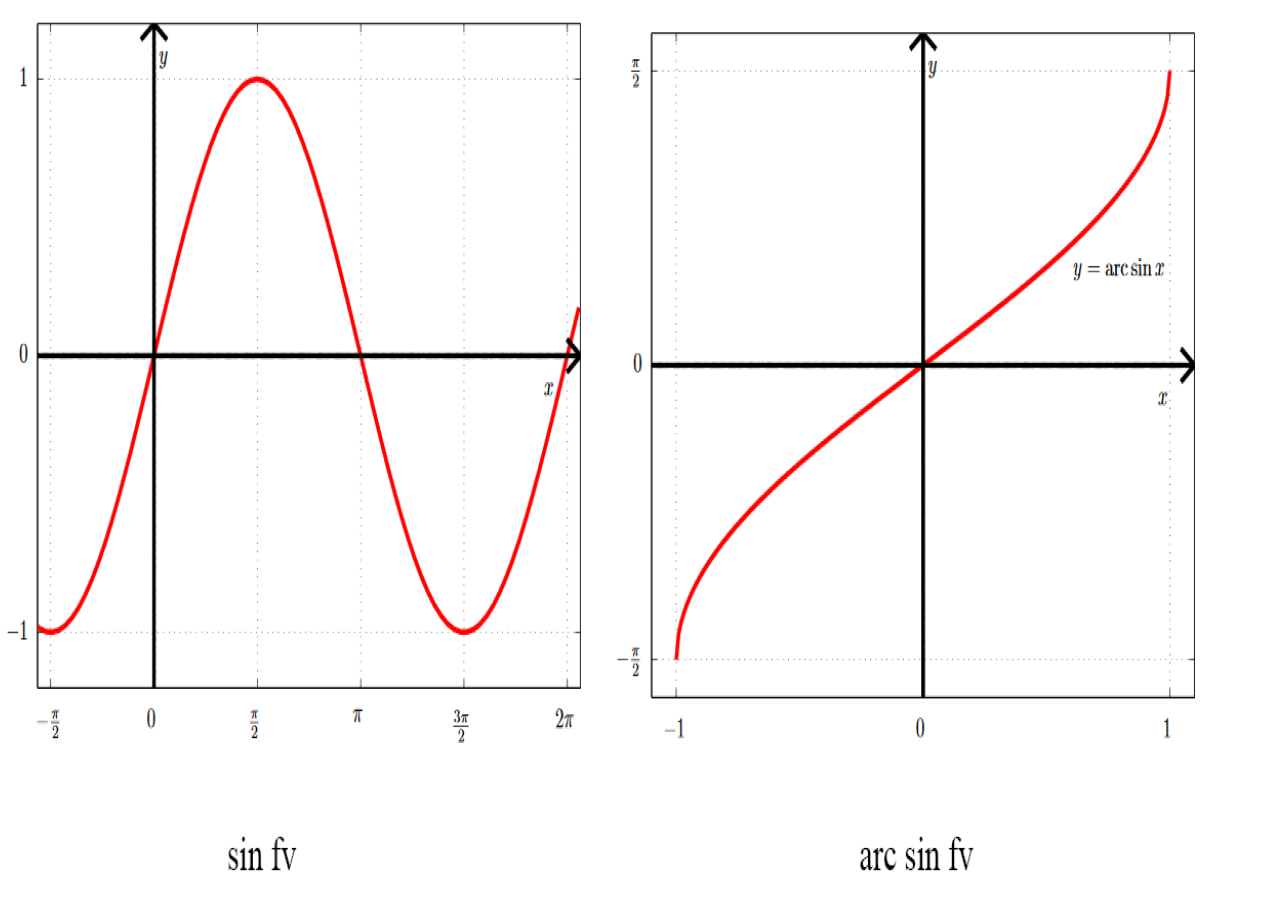
\includegraphics[width=15cm]{kepek/sin.png}
	\item \textbf{Értelmezze az arc tg függyvényt, és ábrázolja egy koordinátarendszerben a tg és az arc tg függvényeket.}\\[0.1cm]A $[-\frac{\pi}{2},\frac{\pi}{2}]$ intervallumon szigorúan monoton ág inverze $\arctan x$. Ez a főág vagy főérték.\\[0.1cm]Ábárzolásuk:\\[0.1cm]
	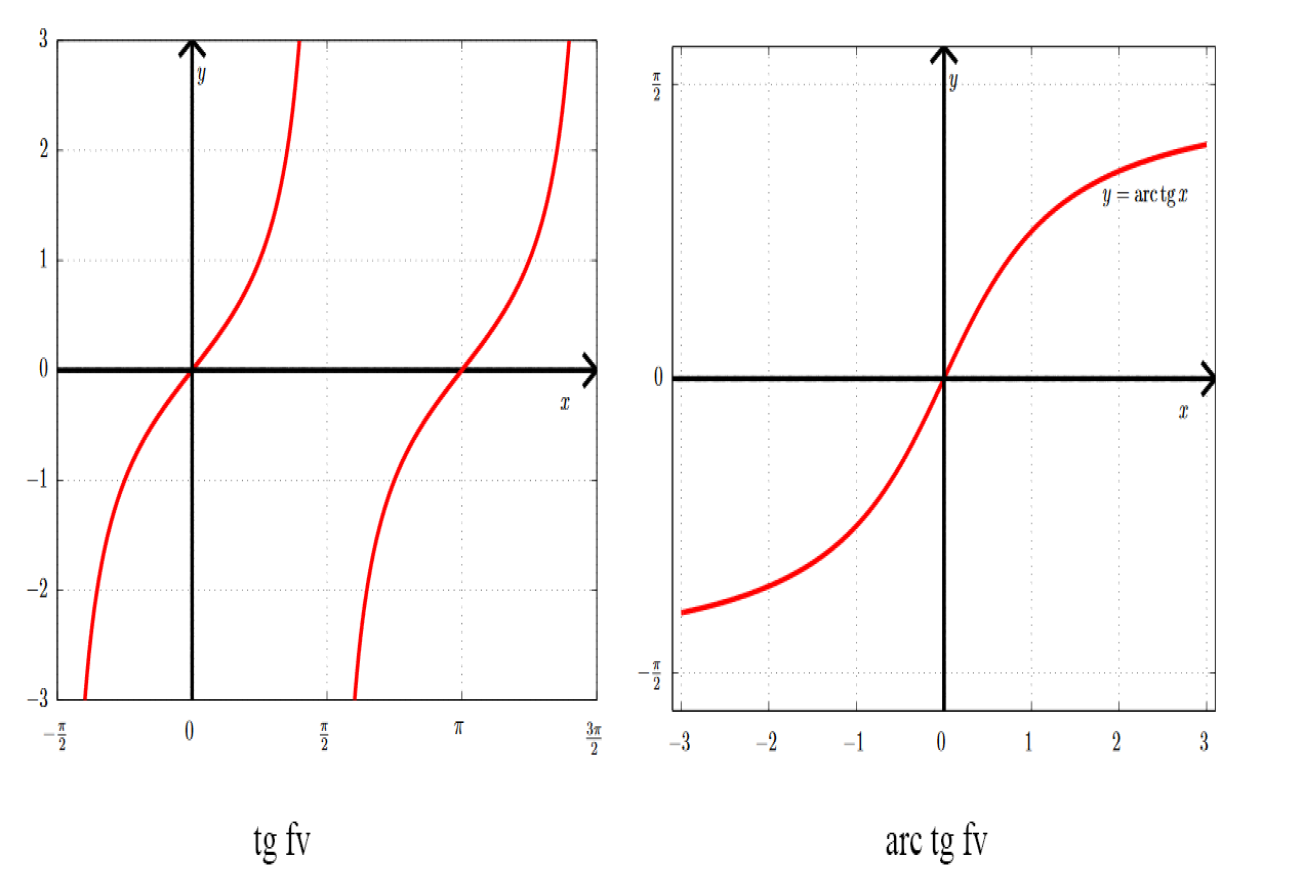
\includegraphics[width=15cm]{kepek/tan.png}
	\item \textbf{Mi a kétszer deriválható függvény fogalma?}\\[0.1cm]$f$ kétszer deriválható $a$-ban, ha $\exists K(a)$, hogy $f\in\D(K(a))$ és $f'\in\D(a)$\\[0.2cm] Jelölés: $f''(a)=(f')'(a),\quad(f\in\D^2(a))$
	\item \textbf{Mi a konvex függvény definíciója?}\\[0.1cm]Az $\fabr$ függvény konvex, ha\\[0.1cm] $\forall x_1,x_2\in(a,b),x_1<x_2,\forall\lambda\in[0,1]: f(\lambda x_1+(1-\lambda)x_2)\leq\lambda f(x_1)+(1-\lambda)f(x_2)$
	\item \textbf{Jellemezze egy függvény \textit{konvexitását} az első derivált segítségével.}\\[0.1cm]$\fabr$ Ha $f\dab$, akkor:\\[0.1cm] $f$ konvex $\Leftrightarrow f'\nearrow\quad(a,b)$-n.
	\item \textbf{Jellemezze egy függvény \textit{konkávitását} a második derivált segítségével.}\\[0.1cm]$\fabr$ Ha $f\in\D^2(a,b)$, akkor:\\[0.1cm] $f$ konkáv $\Leftrightarrow f''\leq0\quad(a,b)$-n.
\end{enumerate}
\end{document}